\section{Classification}
For the goal of classifying simulated data, we have used five different model types,
spanning a range of complexities, architectures, and parameters.
The reason for multiple models is the fundamental difference between the
simulated and experimental datasets; labels. Without ground truth labels
for the experimental data, we need other ways to assess how a model performs in
its task. We attempt to gain some insight by comparing the models' performance on
simulated data with their outputs when applied to experimental data.

We train the models on three sets of simulated data.
The first (a) is the simulated data as-is, with no changes apart from normalization
and pre-processing. The second (b) is the same dataset, but with specific pixels in
the 'detector images' set to zero. These pixels are effectively "dead" in the
experimental dataset, and mimicking this in the simulated data may allow us to monitor
what effect this has on model performance.

\subsection{Simulated data}
In table \ref{tab:classification-simulated-all-f1-auc} the performance of each model 
trained is reported using the f1-score and auc-score. The model architecture for each 
model is described in (ref appendix).
As a benchmark, we are including a state of the art pretrained 
network (\cite{}VGG HERE) applied to the data using the approach described 
in \ref{section:method-pretrained}.
\begin{table}
\centering
\caption{
Test set F1-scores and roc-AUC scores for classification of simulated datausing multiple models.
Models are trained on a) unmodified data, b) data where specific pixels are set to zero to mimic
'dead' pixels in experimental data, and c) same as b) and imbalanced to mimic experimental data. 
Error estimates are the standard deviation in results from k-fold cross-validation with $K=5$ folds.
}
\label{tab:classification-simulated-all-f1-auc}
\begin{tabular}{llllll}
\toprule
{} &                                            Logistic &                                               Dense &                                       Convolutional &                                    Pretrained VGG16 &                                              Custom \\
\midrule
F1-score (a) &  $\underset{\num{+- 7.727e-03 }  }{\num{ 0.738 } }$ &  $\underset{\num{+- 1.329e-02 }  }{\num{ 0.91 } }$ &  $\underset{\num{+- 6.286e-03 }  }{\num{ 0.964 } }$ &  $\underset{\num{+- 1.591e-02 }  }{\num{ 0.911 } }$ &  $\underset{\num{+- 2.260e-02 }  }{\num{ 0.957 } }$ \\
F1-score (b) &  $\underset{\num{+- 2.273e-03 }  }{\num{ 0.732 } }$ &  $\underset{\num{+- 8.276e-03 }  }{\num{ 0.916 } }$ &  $\underset{\num{+- 3.640e-02 }  }{\num{ 0.758 } }$ &  $\underset{\num{+- 1.926e-02 }  }{\num{ 0.897 } }$ &  $\underset{\num{+- 7.601e-03 }  }{\num{ 0.938 } }$ \\
F1-score (c) &  $\underset{\num{+- 8.483e-02 }  }{\num{ 0.292 } }$ &  $\underset{\num{+- 1.233e-01 }  }{\num{ 0.52 } }$ &  $\underset{\num{+- 9.458e-02 }  }{\num{ 0.9 } }$ &  $\underset{\num{+- 3.606e-02 }  }{\num{ 0.823 } }$ &  $\underset{\num{+- 1.047e-01 }  }{\num{ 0.97 } }$ \\
AUC (a)      &  $\underset{\num{+- 6.515e-04 }  }{\num{ 0.832 } }$ &  $\underset{\num{+- 1.774e-02 }  }{\num{ 0.956 } }$ &  $\underset{\num{+- 2.185e-03 }  }{\num{ 0.988 } }$ &  $\underset{\num{+- 8.505e-03 }  }{\num{ 0.956 } }$ &  $\underset{\num{+- 2.218e-02 }  }{\num{ 0.979 } }$ \\
AUC (b)      &  $\underset{\num{+- 9.779e-04 }  }{\num{ 0.832 } }$ &  $\underset{\num{+- 2.604e-03 }  }{\num{ 0.956 } }$ &  $\underset{\num{+- 9.848e-03 }  }{\num{ 0.977 } }$ &  $\underset{\num{+- 9.530e-03 }  }{\num{ 0.949 } }$ &  $\underset{\num{+- 1.763e-03 }  }{\num{ 0.99 } }$ \\
AUC (c)      &  $\underset{\num{+- 1.601e-03 }  }{\num{ 0.832 } }$ &  $\underset{\num{+- 2.750e-03 }  }{\num{ 0.83 } }$ &  $\underset{\num{+- 8.035e-03 }  }{\num{ 0.944 } }$ &  $\underset{\num{+- 4.376e-03 }  }{\num{ 0.92 } }$ &  $\underset{\num{+- 5.312e-04 }  }{\num{ 0.986 } }$ \\
\bottomrule
\end{tabular}
\end{table}

in figure \ref{fig:confmat-simulated}
\begin{figure}
\centering
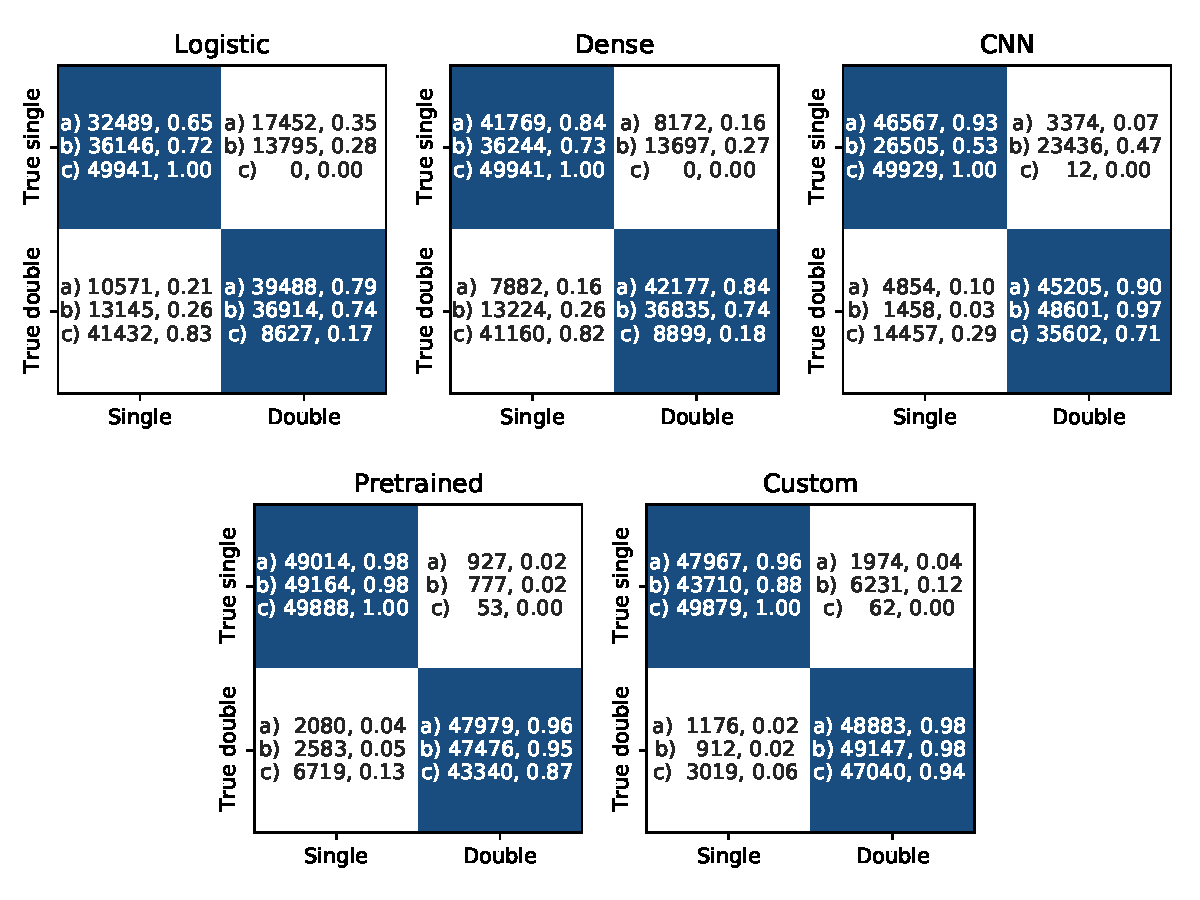
\includegraphics[width=\textwidth]{chapters/results/figures/confmat_simulated.pdf}
\caption{\label{fig:confmat-simulated}Confusion matrices for each model trained
on simulated data. For each model and dataset, the number of events and ratio of each
event type are given. a) unmodified data. b) select pixels set to zero. c) Same as in b)
with the intentionally imbalanced.}
\end{figure}
\subsection{Experimental data}

\section{Regression}
On data already classified, we attempt to predict the energy of the events and the position of origin for
the electrons. Because there is a travel distance between the ejection site and the scintillator array,
the positions aren't necessarily the locations of the highest-intensity pixels in the detector images.
\subsection{Simulated data}
\subsubsection{Position of origin}
\begin{table}
\centering
\caption{
Test set R2-scores for regression of positions of origin on simulated data, with models trained on data with: 
a) no modifications, b) specific pixels set to zero to mimic experimental data, and c) imbalanced dataset
in addition to modifications in b) to further mimic experimental data. Error estimates are the standard deviation 
in results from validation data in k-fold cross-validation with $K=5$ folds.
}
\label{tab:regression-simulated-all-positions-r2}
\begin{tabular}{llllll}
\toprule
{} &                                              Linear &                                               Dense &                                                 CNN &                                           Pretrained &                                              Custom \\
\midrule
Single (a) &  $\underset{\num{+- 2.889e-03 }  }{\num{ 0.8 } }$ &  $\underset{\num{+- 7.007e-04 }  }{\num{ 0.988 } }$ &  $\underset{\num{+- 9.207e-04 }  }{\num{ 0.997 } }$ &  $\underset{\num{+- 2.229e-01 }  }{\num{ 0.997 } }$ &  $\underset{\num{+- 1.366e-04 }  }{\num{ 0.999 } }$ \\
Single (b) &  $\underset{\num{+- 2.749e-03 }  }{\num{ 0.781 } }$ &  $\underset{\num{+- 1.406e-03 }  }{\num{ 0.982 } }$ &  $\underset{\num{+- 1.110e-03 }  }{\num{ 0.98 } }$ &  $\underset{\num{+- 4.513e-04 }  }{\num{ 0.997 } }$ &  $\underset{\num{+- 9.603e-04 }  }{\num{ 0.995 } }$ \\
Single (c) &  $\underset{\num{+- 2.749e-03 }  }{\num{ 0.781 } }$ &  $\underset{\num{+- 1.424e-03 }  }{\num{ 0.982 } }$ &  $\underset{\num{+- 1.080e-03 }  }{\num{ 0.98 } }$ &  $\underset{\num{+- 4.932e-04 }  }{\num{ 0.997 } }$ &  $\underset{\num{+- 1.639e-03 }  }{\num{ 0.993 } }$ \\
Double (a) &  $\underset{\num{+- 3.766e-03 }  }{\num{ 0.37 } }$ &  $\underset{\num{+- 5.601e-03 }  }{\num{ 0.456 } }$ &  $\underset{\num{+- 1.603e-03 }  }{\num{ 0.471 } }$ &  $\underset{\num{+- 1.552e-01 }  }{\num{ 0.29 } }$ &  $\underset{\num{+- 3.467e-04 }  }{\num{ 0.493 } }$ \\
Double (b) &  $\underset{\num{+- 6.815e-04 }  }{\num{ 0.364 } }$ &  $\underset{\num{+- 3.431e-03 }  }{\num{ 0.458 } }$ &  $\underset{\num{+- 1.835e-03 }  }{\num{ 0.435 } }$ &  $\underset{\num{+- 1.550e-01 }  }{\num{ 0.289 } }$ &  $\underset{\num{+- 2.865e-04 }  }{\num{ 0.489 } }$ \\
Double (c) &  $\underset{\num{+- 7.768e-03 }  }{\num{ 0.357 } }$ &  $\underset{\num{+- 9.456e-03 }  }{\num{ 0.417 } }$ &  $\underset{\num{+- 2.507e-03 }  }{\num{ 0.442 } }$ &  $\underset{\num{+- 8.452e-01 }  }{\num{ -0.924 } }$ &  $\underset{\num{+- 4.187e-03 }  }{\num{ 0.478 } }$ \\
\bottomrule
\end{tabular}
\end{table}

\subsubsection{Energy}
\begin{table}
\centering
\caption{
Test set R2-scores for regression of energies on simulated data, with models trained on data with: 
a) no modifications, b) specific pixels set to zero to mimic experimental data, and c) imbalanced dataset
in addition to modifications in b) to further mimic experimental data. Error estimates are the standard deviation 
in results from validation data in k-fold cross-validation with $K=5$ folds.
}
\label{tab:regression-simulated-all-energies-r2}
\begin{tabular}{llllll}
\toprule
{} &                                              Linear &                                               Dense &                                                 CNN &                                          Pretrained &                                              Custom \\
\midrule
Single (a) &  $\underset{\num{+- 3.334e-02 }  }{\num{ 0.932 } }$ &  $\underset{\num{+- 3.623e-02 }  }{\num{ 0.934 } }$ &  $\underset{\num{+- 4.088e-02 }  }{\num{ 0.937 } }$ &  $\underset{\num{+- 3.761e-02 }  }{\num{ 0.926 } }$ &  $\underset{\num{+- 2.997e-02 }  }{\num{ 0.944 } }$ \\
Single (b) &  $\underset{\num{+- 2.459e-02 }  }{\num{ 0.768 } }$ &  $\underset{\num{+- 2.222e-02 }  }{\num{ 0.745 } }$ &  $\underset{\num{+- 2.575e-02 }  }{\num{ 0.48 } }$ &  $\underset{\num{+- 1.948e-02 }  }{\num{ 0.781 } }$ &  $\underset{\num{+- 3.167e-02 }  }{\num{ 0.752 } }$ \\
Single (c) &  $\underset{\num{+- 2.459e-02 }  }{\num{ 0.768 } }$ &  $\underset{\num{+- 2.223e-02 }  }{\num{ 0.745 } }$ &  $\underset{\num{+- 2.522e-02 }  }{\num{ 0.432 } }$ &  $\underset{\num{+- 1.955e-02 }  }{\num{ 0.781 } }$ &  $\underset{\num{+- 2.956e-02 }  }{\num{ 0.724 } }$ \\
Double (a) &  $\underset{\num{+- 3.349e-02 }  }{\num{ 0.49 } }$ &  $\underset{\num{+- 3.084e-02 }  }{\num{ 0.49 } }$ &  $\underset{\num{+- 4.130e-02 }  }{\num{ 0.488 } }$ &  $\underset{\num{+- 3.138e-02 }  }{\num{ 0.489 } }$ &  $\underset{\num{+- 3.618e-02 }  }{\num{ 0.491 } }$ \\
Double (b) &  $\underset{\num{+- 3.157e-03 }  }{\num{ 0.485 } }$ &  $\underset{\num{+- 2.347e-03 }  }{\num{ 0.487 } }$ &  $\underset{\num{+- 7.096e-03 }  }{\num{ 0.478 } }$ &  $\underset{\num{+- 4.508e-03 }  }{\num{ 0.489 } }$ &  $\underset{\num{+- 3.659e-03 }  }{\num{ 0.464 } }$ \\
Double (c) &  $\underset{\num{+- 4.611e-02 }  }{\num{ 0.434 } }$ &  $\underset{\num{+- 4.583e-02 }  }{\num{ 0.422 } }$ &  $\underset{\num{+- 4.554e-02 }  }{\num{ 0.446 } }$ &  $\underset{\num{+- 3.868e-02 }  }{\num{ 0.417 } }$ &  $\underset{\num{+- 4.802e-02 }  }{\num{ 0.401 } }$ \\
\bottomrule
\end{tabular}
\end{table}
